%
% Sección de comparación de desempeño,
% presentación de TT 1.
%
% Proyecto Lovelace.
%

\subsection{Resultados}

\begin{frame}{Resultados}{Comparaciones de desempeño}
  \only<1>
  {
    Las pruebas mostradas a continuación se realizaron en una computadora
    Toshiba S55-B5289 con las siguientes especificaciones:
    \begin{itemize}
      \item Procesador Intel Core i7-4710HQ.
      \begin{itemize}
        \item 6M caché, hasta 3.50GHz.
        \item 8 núcleos.
      \end{itemize}
      \item 8GB de RAM.
      \item En los casos pertinentes, se utilizó AES-NI\footnotemark.
      \item Se utilizó el compilador GCC versión 7.3.1.
      \item Se utilizó GNU gprof 2.30 como herramienta para obtener los
        perfiles de las funciones.
    \end{itemize}
    \footnotetext{
      \textit{Intel Advanced Encryption Standard New Instructions}.
    }
  }
  \only<2>
  {
    {\small
      \begin{table}
        \begin{center}
          \begin{tabular}{c|c|c|}
            \cline{2-3}
            & Tokenización & Detokenización \\
            \hline
            \multicolumn{1}{|c|}{BPS}
              & 0.11   $m$s & 0.11 $m$s   \\\hline
            \multicolumn{1}{|c|}{FFX}
              & 0.12   $m$s & 0.12 $m$s   \\\hline

            \multicolumn{1}{|c|}{TKR}
              & 0.03   $m$s & 0.00 $m$s\footnotemark   \\\hline
            \multicolumn{1}{|c|}{AHR}
              & 48.16  $m$s & 5.80 $m$s   \\\hline
            \multicolumn{1}{|c|}{DRBG}
              & 118.24 $m$s & 10.84 $m$s  \\\hline
          \end{tabular}

          \caption{Comparación de tiempos de tokenización.}
          \label{tabla:tiempos_tokenizacion}
        \end{center}
      \end{table}
    }
    \footnotetext{
      Debido a la resolución de GNU-profiler, la operación de tokenización de
      TKR parece ser, incorrectamente, instánea.
    }
  }

  \only<3>
  {
    \begin{figure}[H]
      \begin{center}
        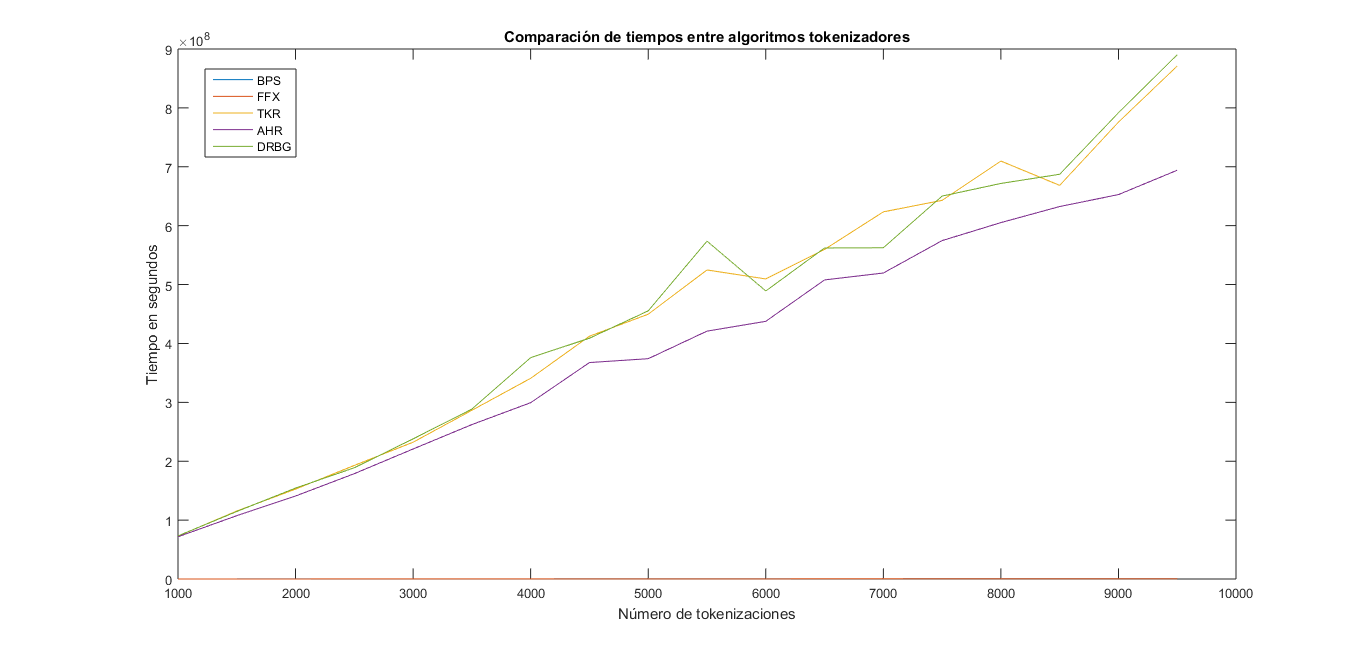
\includegraphics[width=1.0\linewidth]
          {../../../diagramas_comunes/desempenio/tok_todos.png}
        \caption{Tiempos de tokenización generales.}
      \end{center}
    \end{figure}
  }

  \only<4>
  {
    \begin{figure}[H]
      \begin{center}
        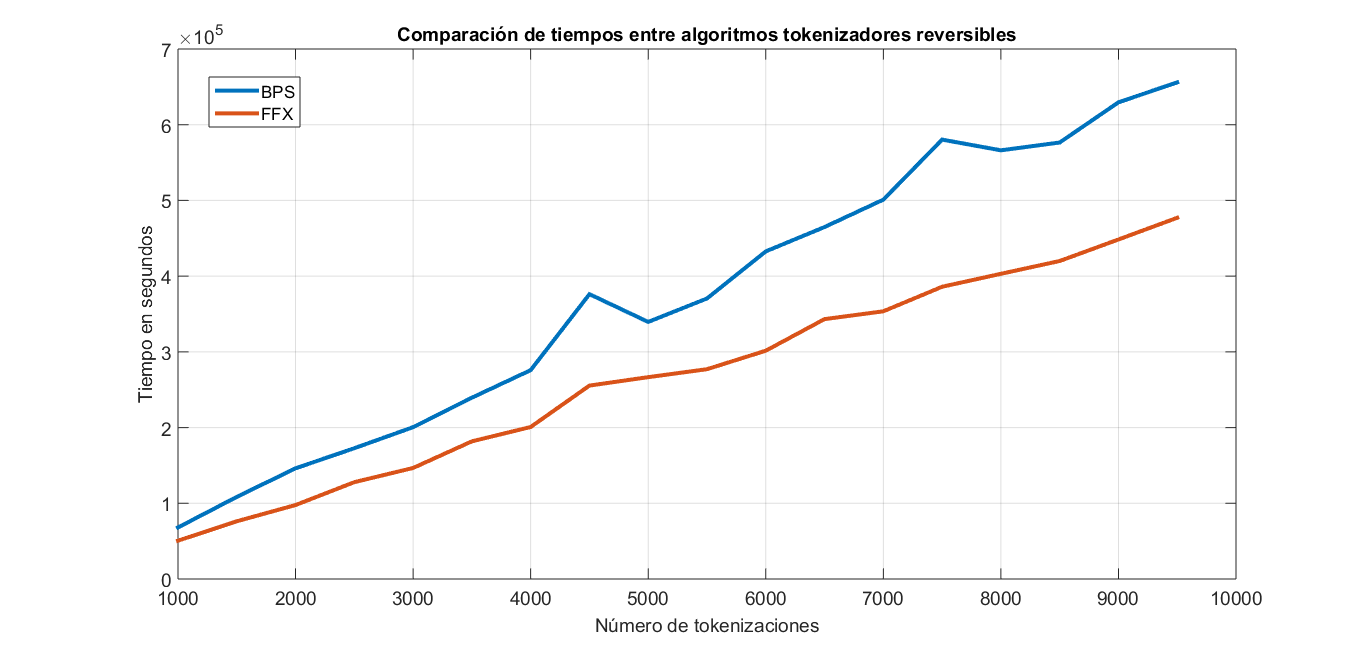
\includegraphics[width=1.0\linewidth]
          {../../../diagramas_comunes/desempenio/tok_rev.png}
        \caption{Tiempos de tokenización de reversibles.}
      \end{center}
    \end{figure}
  }

  \only<5>
  {
    \begin{figure}[H]
      \begin{center}
        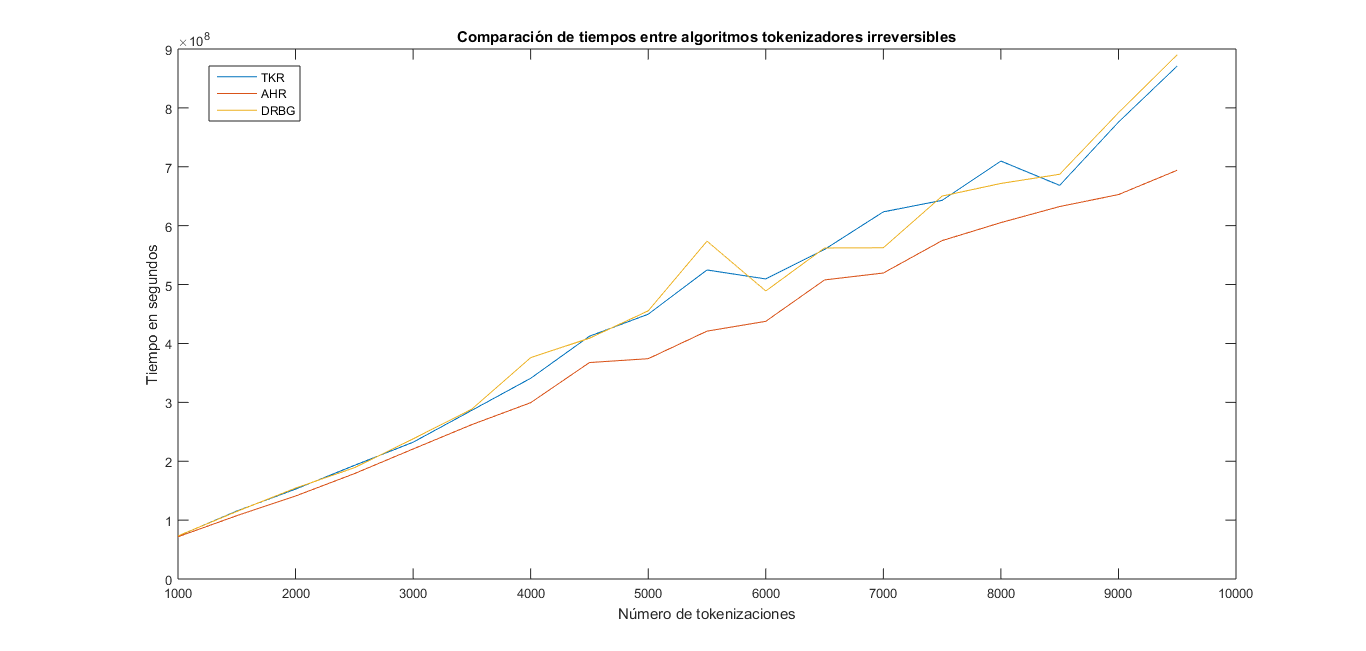
\includegraphics[width=1.0\linewidth]
          {../../../diagramas_comunes/desempenio/tok_irrev.png}
        \caption{Tiempos de tokenización de irreversibles.}
      \end{center}
    \end{figure}
  }

  \note
  {
    Los tiempos de los reversibles son mucho más cortos.

    Las gráficas muestran solo los procesos de tokenización: con la
    detokenización pasan cosas bastante similares.
  }

\end{frame}

\begin{frame}{Resultados}{Pruebas de aleatoriedad}

  En \cite{nist_pruebas} el NIST describe un conjunto de pruebas estadísticas
  que sirven para determinar la aleatoriedad de un generador pseudoaleatorio.
  Se trata de 15 pruebas generales (algunas de ellas con subpruebas) que es
  necesario ejecutar sobre los bits generados.

  Para cada instancia de los generadores implementados se ejecutó el conjunto
  de pruebas 20 veces, cada una con medio millón de bits (un total de veinte
  millones).

  \only<1>
  {
    Resultados para generador basado en función hash:
    \begin{itemize}
      \item 112 bits de seguridad: 14 de 15.
      \item 128 bits de seguridad: 15 de 15.
      \item 192 bits de seguridad: 14 de 15.
      \item 256 bits de seguridad: 15 de 15.
    \end{itemize}
  }

  \only<2>
  {
    Resultados para generador basado en cifrador por bloques:
    \begin{itemize}
      \item 112 bits de seguridad: 15 de 15.
      \item 128 bits de seguridad: 15 de 15.
      \item 192 bits de seguridad: 15 de 15.
      \item 256 bits de seguridad: 15 de 15.
    \end{itemize}
  }

  \note
  {
    Estrictamente hablando, el generador basado en una función hash no es
    totalmente aleatorio, dado que falló en un par de pruebas. Sin embargo,
    el número de veces que se ejecutó el conjunto de pruebas (veinte) es
    un número relativamente pequeño (en comparación con lo recomendado por
    el NIST); esto por los recursos de cómputo que las pruebas exigen.
  }

\end{frame}
